\scanpage{17}
\margin{\unsure{faire le raisonnement}}
\margin{\figure{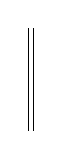
\begin{tikzpicture}\draw (0,0)--(0,1.3);\draw (.07,0)--(.07,1.3);\end{tikzpicture}}}
Alors on voit que $P_{\mathrm{an}}(1_Y)$ est la classe de \unsure{Coh.} sur $X-a$ représenté par la forme diff. $\dfrac{dz}{z}$, et par suite \deleted{\unsure{on a}} si $P_{\mathrm{an}}(1_Y)=\lambda P_{\mathrm{top}}(1_Y)$, on a
\diagram{\begin{tikzcd}[column sep=small,row sep=small]
\lambda={} & \displaystyle\int_C P_{\mathrm{an}}\unsure{(}1_Y) & {}={} & \displaystyle\int_C\frac{dz}{z} & {}=2i\pi \\
& & \begin{gathered}\text{cercle unité }\deleted{\text{\unsure{coord.}}}\\\text{orienté.}\end{gathered}\arrow[ul,bend left=15]\arrow[ur,bend right=15] & &
\end{tikzcd}}
Donc
\[
\boxed{P_{\mathrm{an}}\left(\frac{1}{2i\pi}1_Y\right)=P_{\mathrm{top}}(1_Y)}
\]
\[
\boxed{\left\{\begin{aligned}
P_{\mathrm{top}}(1_Y)&=\frac{1}{2i\pi}P_{\mathrm{an}}(1_Y)\\
P_{\mathrm{an}}(1_Y)&=2i\pi P_{\mathrm{top}}(1_Y)
\end{aligned}\right.}
\]
\figure{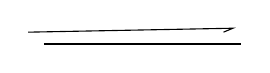
\begin{tikzpicture}\draw (0,0)--(2.6,.05)--(2.48,0);\draw (.2,-.15)--(2.7,-.15);\end{tikzpicture}}

\deleted{\uline{\unsure{Gén.}}} Considérons le diagramme.
\diagram{\begin{tikzcd}[column sep=large,row sep=large]
H^{i+p}_{\unsure{\alpha|Z}}(X,\mathbf Z)\arrow[r,leftrightarrow] &
H^{\deleted{\unsure{*}}\inserted{i}+p}_{\unsure{Z}}(X,\mathbf C)\arrow[r,no head,"\sim","\text{De Rham}" description] &
H^{\deleted{\unsure{*}}\inserted{i}+p}(X,\Omega_X^\bullet)\\
H^{\deleted{\unsure{*}}\inserted{i}}_{\unsure{Z}}(Y,\mathbf Z)\arrow[r]\arrow[u,"P_{\mathrm{top}}"'] &
H^{\deleted{\unsure{*}}\inserted{i}}_{\unsure{Z}}(\deleted{\unsure{X}}\inserted{Y},\mathbf C)\arrow[u,"P_{\mathrm{top}}"']\arrow[r,no head,"\substack{\deleted{\text{\unsure{can.}}}\\\sim}","\frac{1}{(2i\pi)^p}\text{can.}"'] &
\underline{\underline H}^{\deleted{\unsure{*}}\inserted{i}}_{\unsure{Z}}(\deleted{\unsure{X}}\inserted{Y},\Omega^\bullet_{\deleted{\unsure{X}}\inserted{Y}})\arrow[u,"P_{\mathrm{an}}"']
\end{tikzcd}}
\uline{Il est commutatif}, i.e. la formule ci-dessus est valable \uline{globalement}, et en remplaçant $1_Y$ par une classe de Coh. quelc. \unsure{Par raison de la comm. de}
\margin{16}
